\documentclass{tufte-handout}

%\geometry{showframe}% for debugging purposes -- displays the margins

\usepackage{amsmath}

% Set up the images/graphics package
\usepackage{graphicx}
\setkeys{Gin}{width=\linewidth,totalheight=\textheight,keepaspectratio}
\graphicspath{{graphics/}}

\title{Understanding Energy Balance}
\author{Dave Bridges}
\date{}  % if the \date{} command is left out, the current date will be used

% The following package makes prettier tables.  We're all about the bling!
\usepackage{booktabs}

% The units package provides nice, non-stacked fractions and better spacing
% for units.
\usepackage{units}

% The fancyvrb package lets us customize the formatting of verbatim
% environments.  We use a slightly smaller font.
\usepackage{fancyvrb}
\fvset{fontsize=\normalsize}

% Small sections of multiple columns
\usepackage{multicol}

% Provides paragraphs of dummy text
\usepackage{lipsum}

% These commands are used to pretty-print LaTeX commands
\newcommand{\doccmd}[1]{\texttt{\textbackslash#1}}% command name -- adds backslash automatically
\newcommand{\docopt}[1]{\ensuremath{\langle}\textrm{\textit{#1}}\ensuremath{\rangle}}% optional command argument
\newcommand{\docarg}[1]{\textrm{\textit{#1}}}% (required) command argument
\newenvironment{docspec}{\begin{quote}\noindent}{\end{quote}}% command specification environment
\newcommand{\docenv}[1]{\textsf{#1}}% environment name
\newcommand{\docpkg}[1]{\texttt{#1}}% package name
\newcommand{\doccls}[1]{\texttt{#1}}% document class name
\newcommand{\docclsopt}[1]{\texttt{#1}}% document class option name

\begin{document}

\maketitle% this prints the handout title, author, and date

\begin{abstract}
\noindent This lecture will cover the basics of energy balance, including how we sense and measure energy intake and expenditure.  This has very important consequences for understanding weight gain and loss, and understanding how different macronutrients are absorbed, stored and metabolized.
\end{abstract}

\tableofcontents

\pagebreak
\section{Learning Objectives}

\begin{itemize}
\item Apply the concept of energy balance to understanding weight gain and weight loss.
\item Explain the differences in energy content of various macronutrients.
\item Differentiate between the components of energy intake and energy expenditure and evaluate how these contribute to energy balance.
\item Interpret how energy intake and energy expenditure are assessed, including the biases and limitations of these methods.
\item Understand how energy balance and its various sub-components are changed in response to dieting.

\end{itemize}

\section{Key Vocabulary}
\begin{itemize}
	\item Energy Balance
	\item Thermogenesis
	\item Diet-induced Thermogenesis
	\item Resting Energy Expenditure
	\item Exercise Associated Thermogenesis
	\item Metabolic Inefficiency

\end{itemize}

\section{Energy Balance and Changes in Body Weight}

Obesity is now a major epidemic in most societies, with recent estimates showing that in America 38\% of adults and 17\% of children are considered obese\citep{Flegal2016,Ogden2016}.  Fundamentally, people gain weight because of positive energy balance.  This means that if energy intake is larger than energy expenditure, weight (primarily in the form of stored fat) will increase.  This unit will give an overview as to how we define and talk about energy balance (Figure\ref{fig:energy-balance}).

\begin{marginfigure}
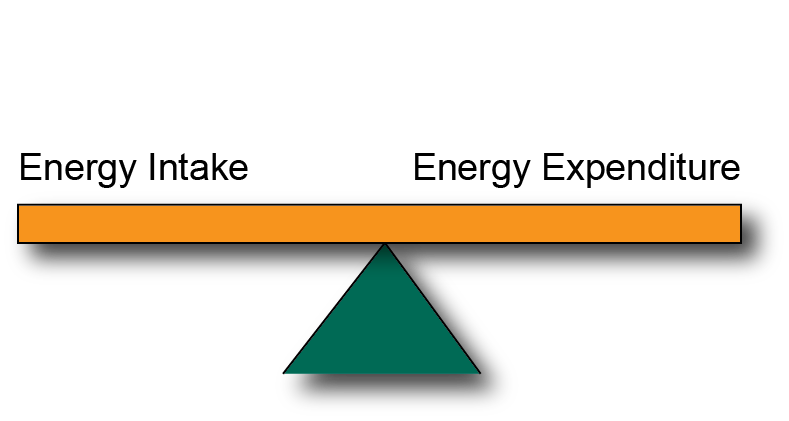
\includegraphics{figures/Energy-Balance.png}\
\caption{Energy balance, when energy expenditure matches energy intake results in no gain or loss of weight.  Positive or negative energy balance occurs when one side increases or the other side decreases.}\label{fig:energy-balance}
\end{marginfigure}

\newthought{It may seem a bit abstract} to think of food, exercise and body weight all in terms of energy, but fundamentally every macronutrient has a different caloric content, and when it is catabolized, that energy is released.  Often some of that energy is passed to another molecule (for example, to ATP) but ultimately all catabolic processes end up generating heat.  The production of heat, known as \emph{thermogenesis}, is an important part of understanding energy balance.  We all have intuitive ideas about someone's metabolic rate whether it be how one person can eat a large meal with no consequences, while another seems to restrict their diet but is unable to lose weight.  Here we will discuss some of the physiology that makes up that energy balance and how this is modified by changes in diet.

\section{Energy Intake}

\subsection{What is Energy Intake?}
Energy intake is the sum of the amount of energy that is taken up by a person.  While a major part of energy intake is the amount of food we eat, a less appreciated aspect is the efficiency\sidenote{In this context, and throughout the course efficiency indicates the percent of energy that is absorbed or used for actions.  Efficiency may be important for an athlete, where nutrients are converted effectively into ATP and then motion.  By the same token, efficiency is the enemy of weight loss, because if macronutrients are efficiently converted in the simplest way to energy, excess calories may be stored.} of nutrient extraction during digestion.  As we will cover in her introduction to digestion, food passes through our bodies and efficient digestion involves extracting as many nutrients as possible from the bolus of food.  Therefore we can consider energy intake as:

\begin{equation}
Energy_{intake} = Energy_{ingested} - Energy_{excreted} - E_{digestion}
\end{equation}

This is important to keep in mind, because different foods have both different energy content and different aptitudes towards being absorbed by the body.  Different people may also have more or less efficiency of nutrient ingestion.  Someone who is malabsorptive, for example may have normal E$_{ingestion}$ but very high E$_{excretion}$ meaning that their E$_{intake}$ is very low.  The energy needed for digestion, is part of what we call Diet-Induced Thermogenesis\sidenote{It is not all of Diet-Induced Thermogenesis however, which also includes the energy released during storage and transport of foods to their eventual destinations}, and is the energy that is expended in the process of digestion.  This could be the breaking of molecular bonds as foods are broken down, or the heat generated by contraction by gastrointestinal smooth muscle cells.

\subsection{How do the foods we eat affect energy intake?}

\begin{margintable}
\centering
\caption{Caloric density of the three major macronutrients and ethanol.  These values are known as Atwater's factors}\label{tab:atwater-values}
\begin{tabular}{cc}
\hline
\textbf{Macronutrient}       & \textbf{Energy Density}                     \\
\hline
Carbohydrates & 4 kcal/g \\
Proteins & 4 kcal/g \\
Lipids & 9 kcal/g \\
Ethanol & 7 kcal/g \\
Fiber & 2 kcal/g \\

\hline
\end{tabular}
\end{margintable}

In general, we know how much energy is contained per gram of each of the major macronutrients (see Table \ref{tab:atwater-values}).  These amounts, were calculated by Atwater and colleagues in the early twentieth century from determining how much heat was produced by burning pure fat, protein or carbohydrates\sidenote{Generally oxygen consumed is calculated rather than heat generated, a method known as indirect calorimetry}.  These values are listed in the nutritional information for many foods.  You might expect that the caloric density of your meal may be calculated by performing indirect calorimetry experiments on these foods.  This is not the case, in general food manufacturers use the composition of their food (in terms of macronutrients) and Atwater's factors to calculate energy density.  This can be misleading, since it refers to the complete energy content of a fuel and not necessarily the amount of calories actually absorbed by a typical person.  

\subsection{How do we assess energy intake?}

The FDA suggests that a normal healthy woman eats 2000 kcal per day (2500 for men).  The ideal way to assess energy intake might be to determine the caloric content of all the foods eaten by a person, for example by indirect calorimetry of an identical meal and then subtracting the energy remaining in feces, while accounting for heat generated during digestion.  This is very difficult to do and is rarely done.   More often, to assess $E_{ingested}$ we generally make use of dietary recall surveys, and then compare the amounts and types of foods to a reference database.  A commonly used Food Frequency Questionnaire can be found here: \url{http://bit.ly/2oucJw8}.  There is substantial debate in the research community regarding the accuracy and biases of the different types of dietary recall assessments.


\section{Energy Expenditure}

The other side of the energy balance coin is energy expenditure, or how calories are used.  While energy intake is difficult to measure, energy expenditure is even harder to measure accurately without specialized equipment.  At a molecular level, increases in energy expenditure mean that heat is generated or an inefficiency is present.  We will discuss several examples of this through the course, but Figure \ref{fig:cori-cycle} illustrates one example.  We will discuss this in more detail when we talk about gluconeogenesis, but this cycle is active during exercise where anaerobic glycolysis generates lactate, which is then converted back to glucose for the muscle.  Each turn through this cycle has a net loss of 4 ATP, but nothing new is generated.  Therefore this pathway is inefficient, in that energy (in this case ATP) is used without anything new being made or stored.  If you had a lot of Cori Cycle activity, you would have increased metabolic inefficiency and therefore caused a higher energy expenditure.

\begin{marginfigure}
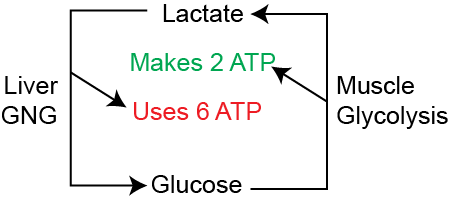
\includegraphics{figures/cori-cycle.png}\
\caption{An inefficient metabolic pathway, the Cori Cycle.  GNG means gluconeogenesis.  Each turn through this cycle uses up 4 ATP (6 ATP used in the liver, 2 generated in the muscle).}
\label{fig:cori-cycle}
\end{marginfigure}


\subsection{What are the components of energy expenditure?}
Energy expenditure can be broken down into several components which add up to one's total daily energy expenditure (TDEE).  This is shown schematically in Figure \ref{fig:tdee-components} taken from a review on the topic \citep{Tam2015}.  These subgroups include the basal metabolic rate (BMR), diet-induced thermogenesis (DIT), non-exercise activity thermogenesis (NEAT) and exercise activity thermogenesis (EAT).  

\begin{equation}
TDEE = BMR + DIT + NEAT + EAT
\end{equation}

\begin{figure}
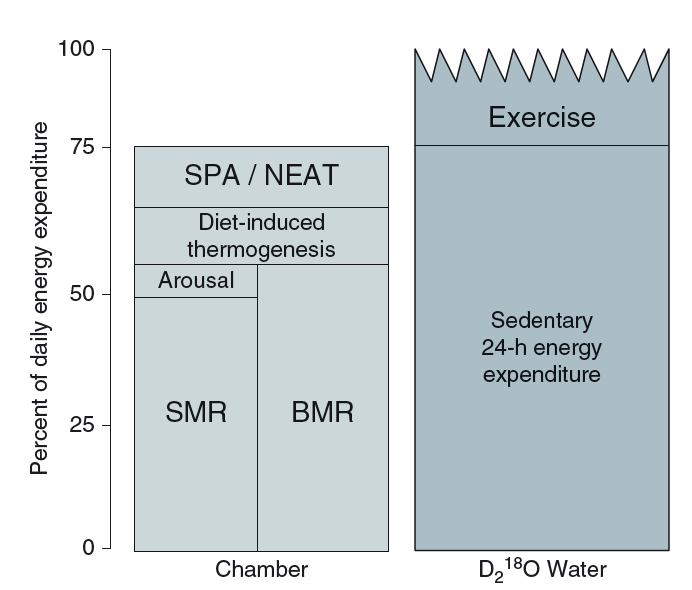
\includegraphics{figures/tdee-components.png}\
\caption{Components of total daily energy expenditure.  SMR represents sleeping metabolic rate. SPA represents spontaneous physical activity.}
\label{fig:tdee-components}
\end{figure}

Each of these components may be affected by genetics, diet, activity levels, sex, and other factors.  What should be apparent from Figure \ref{fig:tdee-components}, is that contrary to many people's intuition, exercise generally comprises only a small portion of total energy expenditure.  To illustrate this, running 5 km may seem like the bulk of your energy expenditure if you went for a run that day, but that expends about 350 Calories, or less than  20\% of your total daily energy expenditure.  

\subsection{How do we calculate energy expenditure}

The major factors that contribute to the BMR are age (declines with age), sex (approximately 11\% higher in males) and body mass, particularly fat-free (or lean) mass.  Up to 85\% of the variance in BMR can be explained by these factors, with a further 11\% being heritable \citep{Bogardus1986a}.  Due to this precision, online calculators are reasonably accurate estimators of energy expenditure.  There are several online calculators available where you can enter your height weight, age and sex to get an estimate.  Try playing around with those numbers to see how they affect estimated energy expenditure.  There are two main ways in which energy expenditure can be experimentally determined.

\newthought{Indirect calorimetry} monitors oxygen consumption and carbon dioxide production, typically over several hours or days.  This can be done in large rooms called metabolic chambers where an individual can live for several days.  The amount of oxygen consumed along with the amount of carbon dioxide produced can be converted into a measure of energy used, in the same way that food combustion can be used to determine the energy content of a meal.  This approach has several advantages, including the fact that DIT, EAT and NEAT can separately be calculated based on whether the individual is currently eating, moving, etc.  The major disadvantage is that the subject has to remain in the room to be monitored and this may not be representative of their normal behaviors.

\newthought{Doubly labeled-water} on the other hand allows the subject to go home and live their normal life, which might be a better approximation of their natural energy expenditure rates.  This technique is based on the differential release of isotopes after a subject drinks radio-labeled water ($^2H_2^{18}O$).  The hydrogen atoms are released only with water, but the oxygen atoms are released as both CO$_2$ and water.  Because of the slower equilibration process it does not provide the temporal resolution of indirect calorimetry, but rather provides an integrated measure of total CO$_2$ production or the time period.  A third experimental method relies on energy conservation and measures E$_{intake}$ and if the subjects are weight stable, E$_{intake}$ should be equal to E$_{expenditure}$. 

\subsection{How does nutrition affect energy expenditure?} 

\newthought{Diet-induced thermogenesis}, also known as the thermic effect of food represents the energy that is used in digestion, absorption and storage of food.  While it only accounts for 5-15\% of TDEE it is the most affected by nutrition choices.  Both meal size (larger, less frequent meals have higher DIT) and macronutrient composition (protein exerts a higher DIT) are major factors in DIT, along with genetics, age, activity levels and insulin sensitivity.  A summary of things that raise the components of energy expenditure can be found in Table \ref{tab:ee-components}.


\begin{table}
\centering
\caption{Components of energy expenditure, and some things that modify their magnitude}
\label{tab:ee-components}
\begin{tabular}{cc}
\hline
\textbf{Component}       & \textbf{Increased By}                     \\
\hline
BMR & Young Age, Male, Lean Mass, Weight Above Set Point\\
EAT & Exercise and Physical Activity\\
DIT & Protein in Meal, Insulin Sensitivity, Meal Size\\
\hline
\end{tabular}
\end{table}


While it was once thought that lower TDEE could be causal of obesity, careful studies in the early 1990s showed that obesity was associated with \emph{higher} energy expenditure rather than lower energy expenditure \citep{Ravussin1982}.  This is now thought to be an adaptive response to gaining weight.  When excess calories are consumed, the body responds by increasing the metabolic rate to try to maintain homeostasis.  Supporting that, during weight loss, the metabolic rate actually \emph{decreases}, likely in an attempt to limit changes in body weight \citep{Leibel1995a}.  This is what is known as a metabolic set point.  It is a metabolic state that the body adapts around.  Unfortunately for those trying to sustain weight loss, this persistent reduction in metabolic rate lasts for many years \citep{Rosenbaum2008}.  Further complicating efforts in weight reduction, studies that have assessed appetite and appetite-driving hormones in successful dieters have shown that there are chronic feelings of both hunger and elevations in hunger hormones, again many years after weight loss \citep{Sumithran2011}.  These two factors, reduced TDEE and increased drive towards energy intake are major reasons why successful weight loss is so difficult to maintain over time.  A schematic of this is shown in Figure \ref{fig:loss-regain}.

\begin{marginfigure}
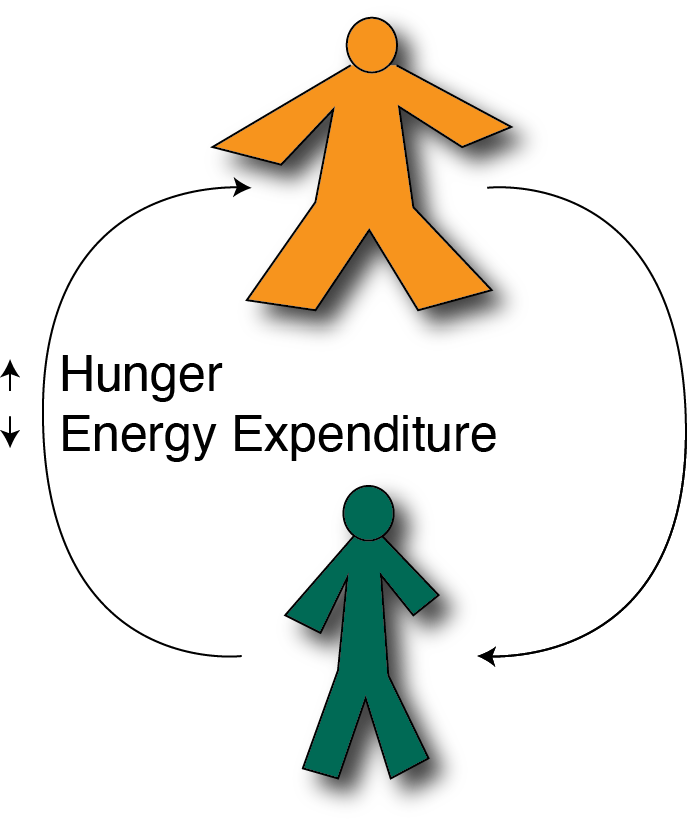
\includegraphics{figures/Loss-Regain.png}\
\caption{Physiological adaptations to weight loss promote weight re-gain.  An individual loses weight, but compensatory decreases in energy expenditure and increases in appetite often result in weight regain.}
\label{fig:loss-regain}
\end{marginfigure}


\bibliography{library}
\bibliographystyle{plainnat}

\end{document}
